\documentclass[border=10pt]{standalone}
\usepackage{pgfplots}
\pgfplotsset{compat=1.18}
\begin{document}
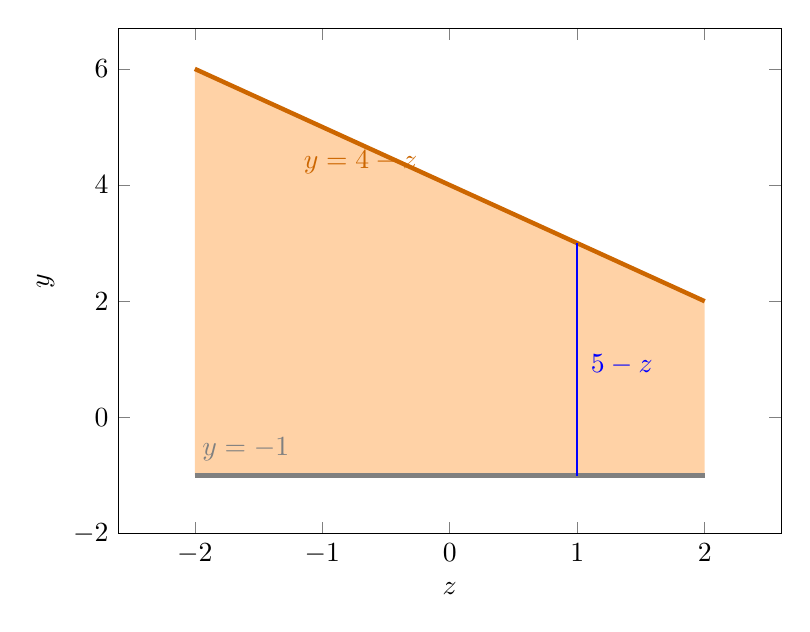
\begin{tikzpicture}
\begin{axis}[
  xlabel=$z$, ylabel=$y$,
  width=10cm, height=8cm,
  xmin=-2.6, xmax=2.6, ymin=-2, ymax=6.7,
]
% the cross-sectional region (trapezoid)
\addplot[fill=orange!35, draw=none] coordinates {(-2,-1) (2,-1) (2,2) (-2,6)} \closedcycle;
% top boundary y = 4 - z
\addplot[orange!80!black, ultra thick, domain=-2:2, samples=2] {4 - x};
% bottom boundary y = -1
\addplot[gray, ultra thick, domain=-2:2, samples=2] {-1};
% a sample vertical slice of length 5-z at z=1
\addplot[blue, thick] coordinates {(1,-1) (1,3)};
\node[blue] at (axis cs:1.35,0.9) {$5-z$};
\node[orange!80!black] at (axis cs:-0.7,4.4) {$y=4-z$};
\node[gray] at (axis cs:-1.6,-0.55) {$y=-1$};
\end{axis}
\end{tikzpicture}
\end{document}
